\documentclass[10pt]{article}
\setlength{\parindent}{0pt}
% \usepackage{setspace} \doublespacing
\usepackage[a4paper, total={6.3in, 9in}]{geometry}
\usepackage{graphicx}
\usepackage{listings}
\usepackage{xcolor}
\usepackage{pdfpages}

% A custom title generation command for physics labs.
\newcommand{\PLtitle}{\setlength{\parindent}{0pt}
\begin{center}

  \huge{\textbf{Lab \Lab: \Ltitle\\}}
  \normalsize 

  Physics 1320L-02 \\
  TA: \TA \\
  Date: \date\\
  Name: \author\\
  
  Team: \team\\


\end{center}
}


\definecolor{codegreen}{rgb}{0,0.6,0}
\definecolor{codegray}{rgb}{0.5,0.5,0.5}
\definecolor{codepurple}{rgb}{0.58,0,0.82}
\definecolor{backcolour}{rgb}{0.95,0.95,0.92}

\lstdefinestyle{mystyle}{
    backgroundcolor=\color{backcolour},   
    commentstyle=\color{codegreen},
    keywordstyle=\color{magenta},
    numberstyle=\tiny\color{codegray},
    stringstyle=\color{codepurple},
    basicstyle=\ttfamily\footnotesize,
    breakatwhitespace=false,         
    breaklines=true,                 
    captionpos=b,                    
    keepspaces=true,                 
    numbers=left,                    
    numbersep=5pt,                  
    showspaces=false,                
    showstringspaces=false,
    showtabs=false,                  
    tabsize=2
}

\lstset{style=mystyle}

% Defining variables for PLtitle
\def\Lab{6}
\def\Ltitle{Capacitors}
\def\author{Kassidy Maberry}
\def\team{Lukas Chavez}
\def\TA{Jonathan Dooley}
\def\date{2024/03/25}
% Defining a variable for creating tabs since writing \hspace*{10mm} is tedious.
\def\tab{\hspace*{10mm}}
\def\halftab{\hspace*{5mm}}

\begin{document}
% Generate title
\PLtitle

% --- Introduction --- % 
\section{Introduction}
\tab Capacitors are devices that are capable of storing electric charge. This is done with two metal plates that
are insulated from eacother storing the charge. One plate will store a positive charge and the other will store a negative charge.
They will continue to hold this charge until the source of electricity is removed. Then the charges will begin to interact with each other
through the insulator.


% --- Methods --- %
\section{Methods}
\tab In this lab we will observe capacitors by sending a charge through four different circuits: A Parallel Connection, Series Connection, Parallel Plate capacitor and
a Cylindrical Capacitor. We will assemble the parallel connection and a series connection. Then to determine the capacitance of each of the circuits we will use an LCR meter and record the current the LCR reads.
This will provide us a reading in farads.\\

% --- Data --- %
\section{Data}

Data obtained for the effective capacitance:
\begin{table}[!h]\label{Table 1}
  \begin{center}
    \begin{tabular}{|c|c|}
      \hline
      Circuit & Capacitance (pF) \\
      \hline
      Capacitor 1    & 10.332                     \\
      \hline
      Capacitor 2    & 91.03          \\
      \hline
      Series circuit     & 9.280                    \\
      \hline
      Parallel circuit     & 101.36                 \\
      \hline
    \end{tabular}
    \caption[short]{Measurements of capacitance of various circuits.}
  \end{center}
\end{table}

Data obtained for Parrallel Plate Capacitor:
\begin{table}[!h]\label{Table 2}
  \begin{center}
    \begin{tabular}{|c|c|c|c|}
      \hline
      Measurement & distance (cm) & Capacitance (pF) & Air Capacitance (pF) \\
      \hline
      1    &  0.435 & 137.57 &     64.80              \\
      \hline
      2    &  0.315     & 219.4&   93.48 \\
      \hline
      3     &      0.640    & 123.43 &  51.71         \\
      \hline
      4     &    1.095    & 86.63 &     36.08     \\
      \hline
      5     &     1.300   & 75.62 &       32.28   \\
      \hline
      6     &    1.025    & 87.45 &       37.33   \\
      \hline
    \end{tabular}
    \caption[short]{Measurements of capacitance of a parrallel circuit.}
  \end{center}
\end{table}

Measurement of Cylindrical Capacitor\\
$d_{i} = 1.26$cm\\
$d_{o} = 2.25$cm\\
$L = 1.22$m\\
$C = 163.42$pF\\

% --- Analysis --- %
\section{Analysis}
\subsection*{Effective Capacitance}

To determine the theoretical capacitance of the parrallel 
circuit we will use Equation~\ref*{SCC}

\begin{equation}\label{SCC}
  C_{eff} = C_{1} + C_{2}
\end{equation}

Plugging in we get a $C_{eff} = 101.362$pF.\\
Then to determine the theoretical capacitance of the series 
circuit we will use Equation~\ref{PCC}.\\

\begin{equation}\label{PCC}
  \frac{1}{C_{eff}} = \frac{1}{C_{1}} + \frac{1}{C_{2}}
\end{equation}
We will need to rearrange this equation to solve for $C_{eff}$.\\
$C_{eff} = \frac{1}{\frac{1}{C_{1}} + \frac{1}{C_{2}}}$

Plugging in we get a $C_{eff} = 9.26$pF.\\

Comparing to our measured values we see that the
measurements are close to the theoretical values.
Calculating the percent error using Equation~\ref{Pe}.\\

\begin{equation}\label{Pe}
  P_{e} = \frac{|P_{theoretical} - P_{measured}|}{P_{theoretical}} * 100 \%
\end{equation}

Giving us a percent error for the parrallel capacitor $P_{e} = 0.002\%$.\\
Then giving us a percent error for the parrallel capacitor $P_{e} = 0.22\%$.\\
Seeing how low the percent error for both this could be assumed to be the inaccuracy of our
measurement devices.\\
\newpage
\subsection*{Parallel Plate Capacitor}

% 1.Plot the capacitance of acrylic, Cacrylic, versus the capacitance of air, Cair.
First let's plot the Capacitance of the air vs the acrylic. 
Plotting this we get the following figure.

\begin{figure}[ht]\label{Graph}
  \begin{center}
    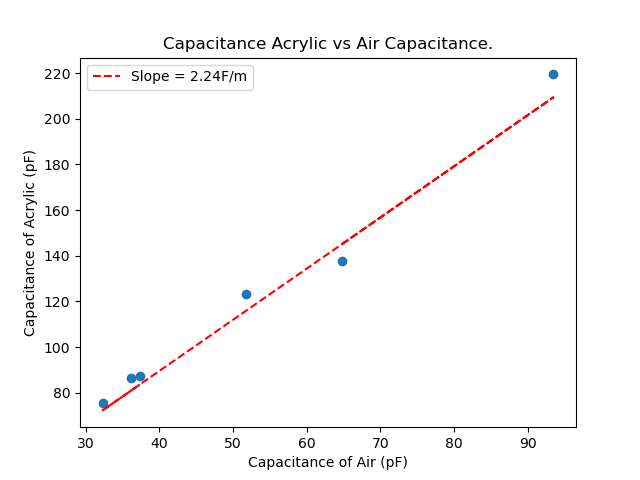
\includegraphics[scale=.50]{capplot.png}
    \caption[short]{Plot of air capacitance vs acrylic capacitance in the parrallel plate capacitor. Generated with Python code shown in the appendix section.}
  \end{center}
\end{figure}
% \newpage

% 2.Use this plot and Equation 4 to determine the dielectric constant, κ, for acrylic. (Try to figure it
% out yourself first, then ask your instructor as needed.) Be sure to explain your work.
To determine the dielectric constant we will use Equation \ref*{dik}
\begin{equation}\label{dik}
  C = k\epsilon_{o}\frac{A}{d}
\end{equation}
As the only variable in this equation that changes is k. Then the dielectric constants
can be written as a ratio of the capacitance. Giving us equation \ref*{dikr}
\begin{equation}\ref*{dikr}
  \frac{C_{acrylic}}{C_{air}} = \frac{k_{acrylic}}{k_{air}}
\end{equation}
As we know the dielectric constant of air is $k_{air} = 1$F/m then our equation is now.\\
\begin{equation}
  \frac{C_{acrylic}}{C_{air}} = k_{acrylic}
\end{equation}
Taking our average capacitances and solving for k we get. $k_{acrylic} = 2.32$F/m another way
we can determine this is by determining the slope of our trendline. Giving us another $k_{acrylic} = 2.24$F/m.
We will take the average of these two giving us a final $k_{acrylic} = 2.28$F/m.\\
\subsection*{Cylindrical Capacitor}

% 1.Find the theoretical value for the capacitance of the cylindrical capacitor

% 2.Compare the theoretical and experimental values of capacitance for the cylindrical capacitor using
% percent error.


% 3.Use Gauss's Law to outline the derivation of the concentric cylinder capacitor without dielectric
% eq(5).


% --- Questions --- %
\section{Questions}

% --- Conclusion --- %
\section{Discussion and Conclusion}


% --- Appendix
\section*{Appendix}\newpage
\includepdf[pages={1-3}]{Data.pdf}


% Insert PDF
\end{document}